\section{编码手册、检索式与报告核查清单}
\label{app:codebook}

\subsection{证据编码手册}
每个研究--要求对仅编码一次，依据该研究针对该要求的主要发现，且针对\cref{sec:intro}所定义的\emph{检测器}用途；裁决者用途一律不予编码。
\begin{description}[leftmargin=1.2em,itemsep=2pt]
  \item[S（支持）] 主要结果显示，在研究自身条件下，类型化模型履行该功能的表现至少与其对照相当；或在无对照时，达到研究所声明的标准；且无需研究额外附加任何条件（本地阈值拟合、重新校准、限定于某种语言或领域、人工审查）。示例：一个开源类型化诈骗检测器不劣于 LLM 评估器~\cite{arx23959}。
  \item[Q（有条件）] 主要结果在不同任务或子类型间不一，或成功取决于研究必须附加的条件。示例：零样本排序表现良好，但阈值必须在本地拟合~\cite{arx29429}。
  \item[N（不支持）] 主要结果显示类型化模型未能履行该功能（相当比例的攻击成功、排序倒置、系统性偏倚、研究认为不可用的校准、门控无法拦截的高置信错误），或明显逊于其对照。示例：替换定义导致判定退化或反转~\cite{arx26758}。
\end{description}
判定规则：（i）若正面与负面发现均为主要发现，编码为 Q；（ii）同一研究针对不同要求可有不同编码；（iii）非实证条目以及未测量任何类型化模型的条目予以记录，但不计入计数；（iv）构成某项要求之检验本身的条件（G2 的对抗性内容，G3 的名称、顺序或语言扰动，G6 的对抗性选取条目）不属于附加条件，因此在这些条件下的失败编码为 N，而需要检验之外条件才能成功的情形编码为 Q。
综合按照 SWiM 指南~\cite{campbell2020swim}统计每项研究主要结果的方向，不合并效应量。
对每一行，我们还记录所测量的系统（托管、开源、二者兼有）、所报告的\jev{}版本，以及在该要求上相对于任何生成式对照的结果（更好、相近、更差、不一、无），并附一句话理由和定位信息。
编码计的是研究数量，并非效应量。

\subsection{设计评价}
每项已编码研究评价三项条目：独立性（独立、作者评估自己构建的系统、与厂商有关联）；设计（预注册；留出评估、交叉验证或重复运行；单次运行；案例研究；非实证）；以及样本量与不确定性的报告情况（样本量并附区间或检验、仅样本量、均无）。
\emph{设计较强}：预注册或留出设计，报告样本量并附区间或检验，且所评估系统非作者自建；\emph{设计较弱}：单次运行、案例研究、非实证，或既未报告样本量也未报告不确定性；\emph{中等}：其余情形。

\subsection{检索式}
\label{app:queries}
\paragraph{arXiv。}
全部检索式均针对 \texttt{export.arxiv.org/api/query} 执行，按投稿日期排序，执行日期为 2026 年 10 月 1 日并于 10 月 4 日重新执行（早期数据集发布依据的是 9 月 28--29 日对两个追踪列表的查阅和网络检索）；\texttt{scripts/rerun\_arxiv\_search.py} 可复现该检索：
\begin{itemize}[nosep,leftmargin=1.5em]
  \item \nolinkurl{all:Jev}
  \item \nolinkurl{abs:"typed decision"}
  \item \nolinkurl{abs:"System One"}
  \item \nolinkurl{abs:RLCD}
  \item \nolinkurl{abs:"calibrated decisions"}
  \item \nolinkurl{abs:"typed answers"}
  \item \nolinkurl{abs:"TypeSafe"}
  \item \nolinkurl{abs:"decision model" AND abs:typed}
  \item \nolinkurl{abs:"System One model"}
  \item \nolinkurl{abs:"System-One"}
  \item \nolinkurl{abs:"direct-decision"}
  \item \nolinkurl{abs:Laya AND abs:decision}
  \item \nolinkurl{abs:"typed probabilistic"}
  \item \nolinkurl{abs:"decision model" AND abs:calibrated}
  \item \nolinkurl{abs:"this-that"}
  \item \nolinkurl{abs:"Reinforcement Learning for Calibrated"}
  \item \nolinkurl{abs:"typed decisions"}
  \item \nolinkurl{abs:"single-pass decision"}
\end{itemize}

\paragraph{Zenodo。}
于 2026 年 10 月 1 日针对 \texttt{zenodo.org/api/records} 执行：
\begin{itemize}[nosep,leftmargin=1.5em]
  \item \nolinkurl{"Jev" AND (TypeSafe OR decision OR "System One")}
  \item \nolinkurl{"System One model"}
  \item \nolinkurl{"typed decision"}
  \item \nolinkurl{"calibrated decisions"}
  \item \nolinkurl{RLCD}
  \item \nolinkurl{title:Jev}
  \item \nolinkurl{title:JEV}
  \item \nolinkurl{description:"TypeSafe"}
  \item \nolinkurl{"Jev" AND (calibration OR typed OR noul)}
  \item \nolinkurl{Laya AND "decision model"}
  \item \nolinkurl{"System One" AND (typed OR calibrated) AND decision}
\end{itemize}


\subsection{筛选与 PRISMA 核查清单}
\label{app:prisma}
\Cref{fig:prisma} 展示了筛选流程。
10 月 4 日的 arXiv 检索返回 955 条记录（去重后 606 条），其中 89 条的日期在发布之日或之后。
在这 89 条中，63 条已在 10 月 1 日首次检索后纳入，另有 1 条当时已在全文阶段排除（其 PDF 为另一份稿件）。
其余 25 条进行了筛选：5 条在标题阶段、4 条在摘要阶段因名称冲突或未涉及类型化模型而被排除；16 条进行了全文阅读，其中 1 条因其“Jev”是一个无关的生成式模型而被排除。
有两篇纳入论文是通过追踪列表而非检索式发现的；其中一篇未测量任何类型化模型，作为背景文献处理。
在 Zenodo 上，约 330 条记录经标题和描述筛选；62 条符合关键词与日期标准；21 条因重复（6 条）、配套存档（5 条）、主题无关（9 条）或不含类型化模型（1 条）而被剔除；其余 41 条中有 13 条为未经评估的应用或工具；在全文阅读的 28 条记录中，有 1 条不含类型化模型。
灰色文献来源来自追踪列表和网络检索；两篇无原始测量的评论作为背景引用。

\paragraph{10 月 8 日的更新检索。}
由于 API 返回 HTTP~429，同样的 18 条 arXiv 检索式改经 arXiv 的高级检索界面执行。每条检索式读取一页结果，每页至多 200 条记录；返回记录最多的一条为 91 条（各检索式的命中数见 \nolinkurl{data/search_rerun_2026-10-08_query_hits.csv}），因此没有检索式被截断，但网页界面与 API 是不同的检索后端。这些检索式共检索到 125 条日期在发布之日或之后的去重记录，其中 46 条不在语料库中。在这 46 条中，10 条已于 10 月 4 日被排除，4 条在标题或摘要阶段被排除；32 条进行了全文阅读，其中 1 条被排除、31 条予以保留，保留者中有 5 条的日期位于主窗口内。
11 条 Zenodo 检索式返回 62 条日期在发布之日或之后的记录，其中 44 条不在已纳入记录之列。由于 10 月 1 日的筛选只保留了数量，这 44 条全部重新筛选；这一重新筛选集合并未列入书面方案，是在编码开始后才加入的。在这 44 条中，7 条为已纳入研究的配套存档，3 条与语料库中已有的 arXiv 记录重复，5 条在标题（2 条）或摘要（3 条）阶段被排除；29 条进行了全文阅读，其中 4 条被排除、25 条予以保留；另有 1 条记录经由配套链接发现并进行了全文阅读。
两个追踪列表未列出任何新的、含原始测量的灰色文献来源；一个仅含厂商内容的页面被排除。
总计全文阅读了 62 个来源，其中 5 个在该阶段被排除；在保留的 57 个中，48 个予以编码，6 个作为背景，2 个为非实证条目，1 个因不含对类型化模型的评估而在编码阶段被排除（\cref{tab:catalogue-update}）。记录及理由见 \nolinkurl{data/search_rerun_2026-10-08.csv}、\nolinkurl{data/search_rerun_zenodo_2026-10-08.csv} 和 \nolinkurl{data/excluded_records_update_2026-10-08.csv}。

\begin{figure}[!htbp]
\centering
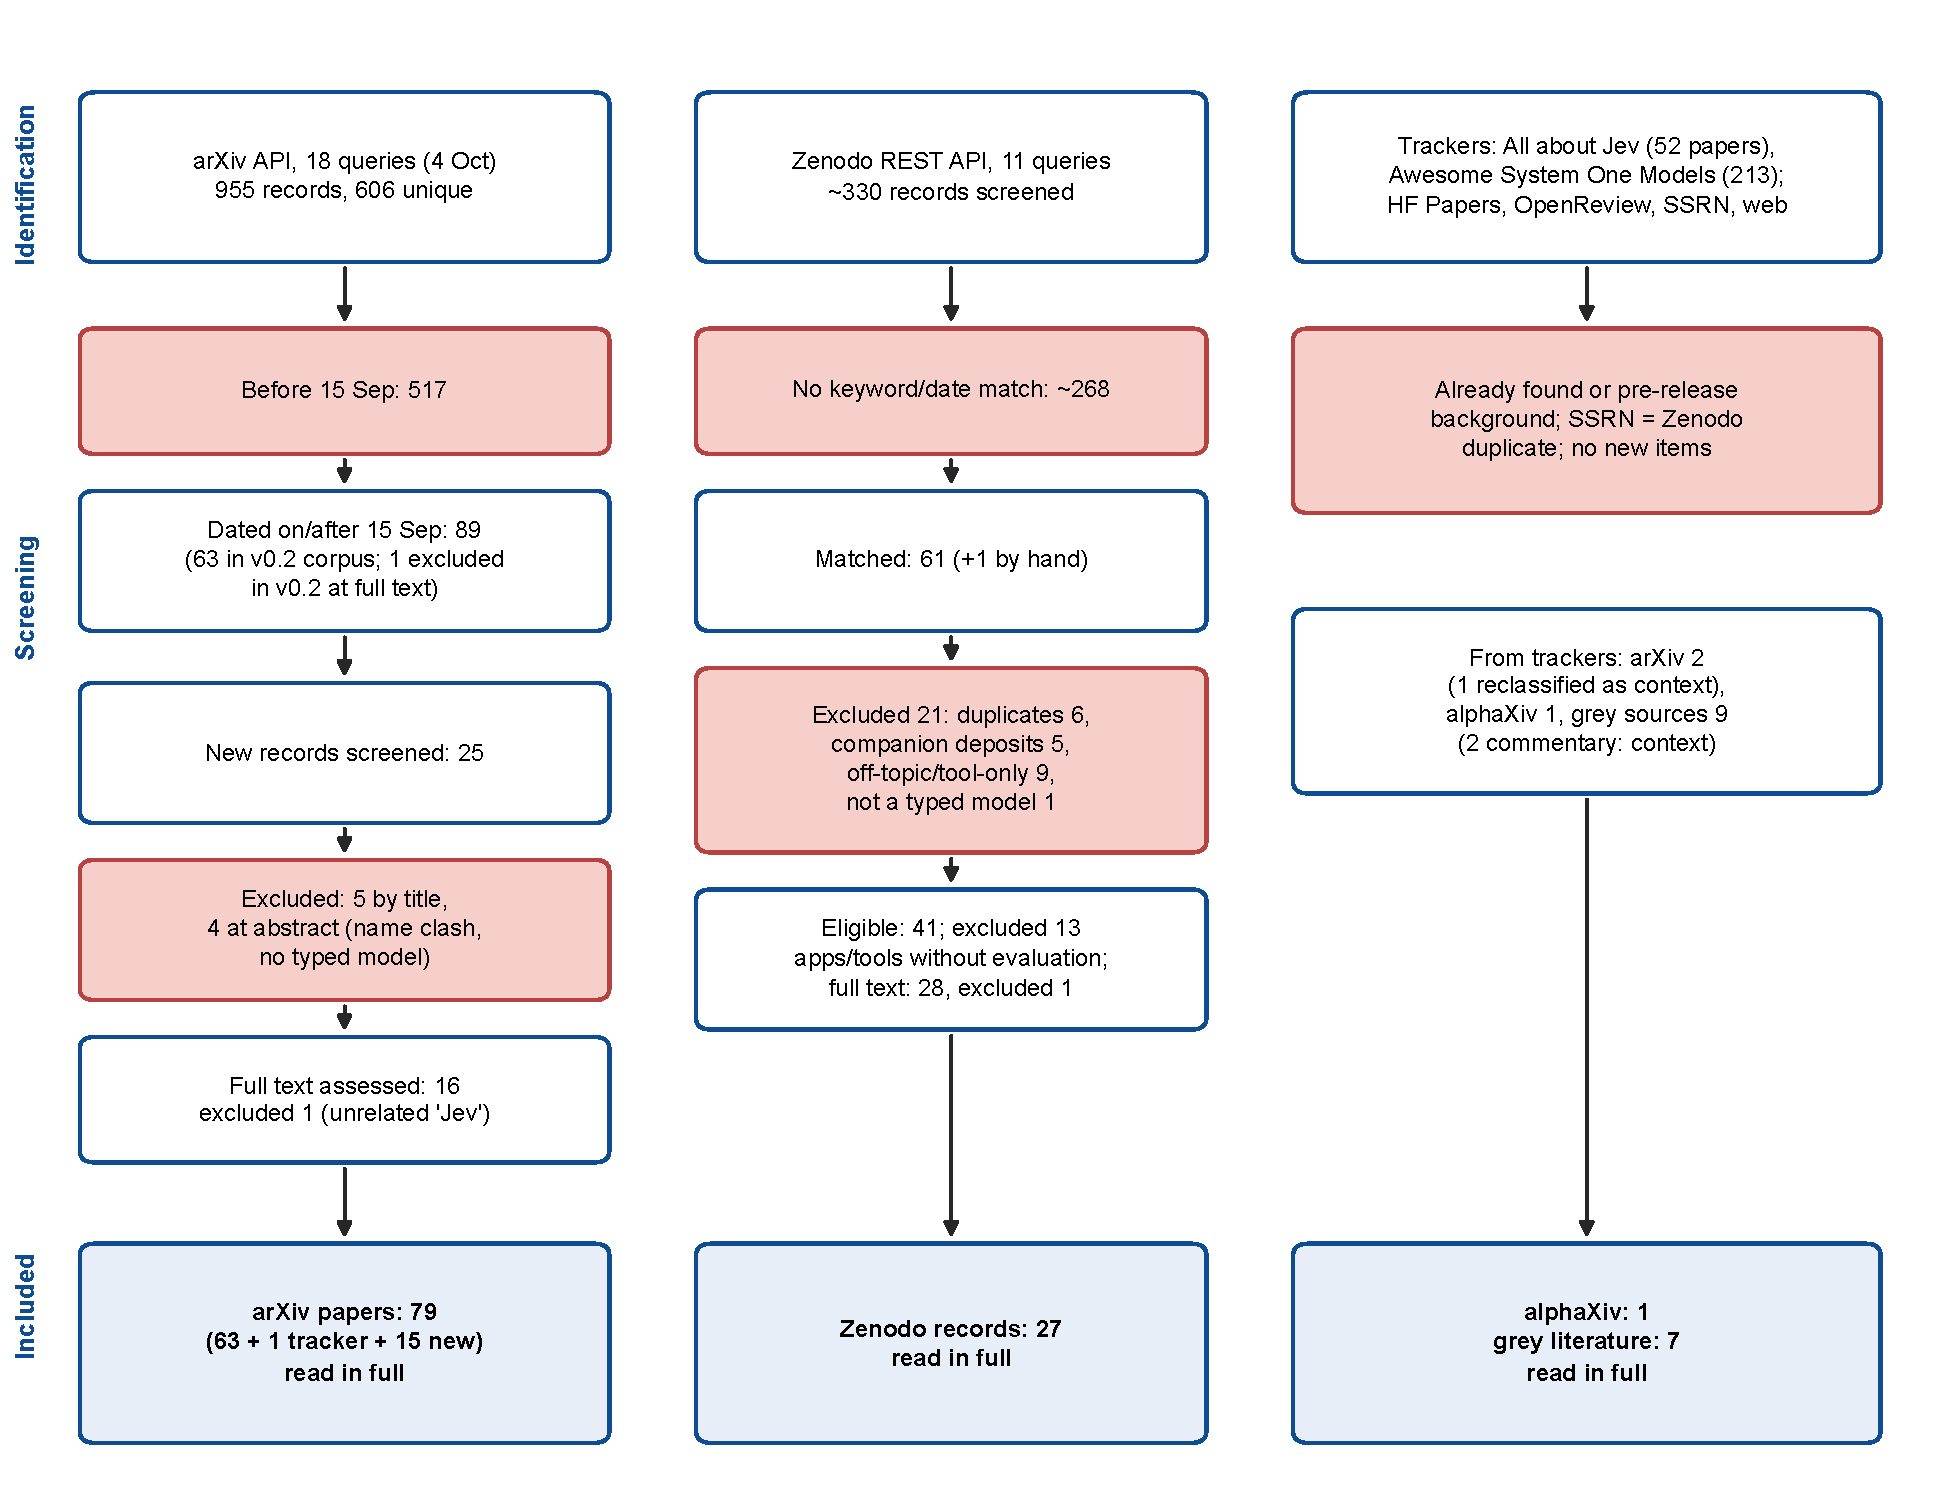
\includegraphics[width=0.85\linewidth]{figures/fig_prisma.pdf}
\caption{按来源划分的识别、筛选与纳入（PRISMA 2020 流程）。由于 API 返回的结果集相互重叠，Zenodo 在第一步的计数为近似值。}
\label{fig:prisma}
\end{figure}

\paragraph{PRISMA 2020 核查清单。}
\Cref{tab:prisma} 将 PRISMA~2020 声明的条目~\cite{page2021prisma}与本文内容逐一对应；未执行的条目均如实注明。

\begingroup
\small
\renewcommand{\arraystretch}{1.15}
\begin{longtable}{@{}p{0.30\linewidth}p{0.64\linewidth}@{}}
\caption{PRISMA 2020 条目及其报告位置。}\label{tab:prisma}\\
\toprule
条目 & 报告位置或状态 \\
\midrule
\endfirsthead
\toprule
条目 & 报告位置或状态 \\
\midrule
\endhead
\bottomrule
\endfoot
标题（1） & 按设计未遵循：本文是一项政策分析，其证据部分在\cref{sec:method}中被界定为结构化快速证据评估 \\
摘要（2） & 摘要陈述了问题、来源、方法、主要结果、确定性及其意义 \\
理由、目的（3--4） & \Cref{sec:intro}（研究问题） \\
纳入标准（5） & \Cref{sec:method}，纳入标准 \\
信息来源、检索（6--7） & \Cref{sec:method}；\cref{app:queries}；\nolinkurl{scripts/rerun_arxiv_search.py} \\
筛选过程（8） & \Cref{sec:method}（评审者与工具）：AI 智能体；无人工重复筛选 \\
数据收集、数据条目（9--10a/b） & \Cref{sec:method}，数据提取；\nolinkurl{data/evidence_coding.csv} \\
研究偏倚风险（11） & 设计评价（\cref{sec:appraisal}）；\nolinkurl{data/quality_appraisal.csv} \\
效应指标（12） & 不适用：按要求统计主要结果的方向；无合并效应 \\
综合：各项综合的纳入资格（13a） & 针对某项要求编码的研究（\cref{app:evidence}） \\
综合：数据准备（13b） & 编码与对照比较字段来自数据提取；未作转换 \\
综合：列表与展示（13c） & \Cref{fig:framework}、\cref{tab:keyfindings}与\cref{tab:evidence} \\
综合：方法（13d） & 按照 SWiM~\cite{campbell2020swim}对方向进行计票；未作 Meta 分析 \\
综合：异质性（13e） & 未作正式分析；任务和模型的异质性在\cref{sec:evidence}中描述 \\
综合：敏感性分析（13f） & 仅纳入设计较强的研究；排除 Zenodo 记录（\cref{sec:across}） \\
报告偏倚（14） & 未作正式评估；在\cref{sec:discussion}中讨论 \\
确定性评估（15） & GRADE 式规则（\cref{sec:appraisal}）；\cref{tab:keyfindings} \\
研究筛选（16a） & \Cref{fig:prisma} \\
看似符合条件但被排除的研究（16b） & \nolinkurl{data/excluded_records.csv}（例如无关的“Jev”论文、PDF 不符的记录以及不含类型化模型的测试框架论文） \\
研究特征（17） & \Cref{app:evidence,app:catalogue} \\
各研究的偏倚风险（18） & \Cref{tab:evidence}；\nolinkurl{data/quality_appraisal.csv} \\
单项研究结果（19） & \Cref{sec:evidence}；理由见 \nolinkurl{data/evidence_coding.csv} \\
综合结果（20a--d） & \Cref{sec:evidence,sec:across}；\cref{fig:framework}；未作异质性分析与正式检验 \\
报告偏倚（21） & 未作正式评估（\cref{sec:discussion}） \\
证据确定性（22） & \Cref{tab:keyfindings} \\
讨论（23a--d） & \Cref{sec:discussion}（解释、证据与过程的局限、意义） \\
注册与方案（24a--c） & 未注册；未发布方案；相对于早期发布的变更见\cref{sec:method} \\
资助（25） & 无资助 \\
利益冲突（26） & 立场声明与利益冲突声明 \\
数据、代码和材料的可获得性（27） & 数据与代码可获得性声明 \\
\end{longtable}
\endgroup
